\documentclass[onecolumn, oneside, letterpaper, draftclsnofoot, 10pt, compsoc]{IEEEtran}

\usepackage[english]{babel}
\usepackage{graphicx}
\usepackage{url}
\usepackage{setspace}
\usepackage{subcaption}

\usepackage{amssymb}
\usepackage{amsmath}
\usepackage{amsthm}
\usepackage{alltt}
\usepackage{color}
\usepackage{enumitem}
\usepackage{textcomp}
\usepackage{cite}

%\usepackage[T1]{fontenc}
\usepackage[utf8]{inputenc}
\usepackage{lmodern}
\usepackage[hidelinks]{hyperref}
\usepackage[normalem]{ulem}

\usepackage[margin=0.75in]{geometry}

\parindent = 0.0 in
\parskip = 0.0 in

% 1. Fill in these details
\def \CapstoneTeamName{         Beaver Hawks}
\def \CapstoneTeamNumber{       14}
\def \GroupMemberOne{           Anton Synytsia}
\def \GroupMemberTwo{           Matthew Phillips}
\def \GroupMemberThree{         Shanmukh Challa}
\def \GroupMemberFour{          Nathan Tan}
\def \CapstoneProjectName{      American Helicopter Society Micro Air Vehicle Competition}
\def \CapstoneSponsorCompany{   Potentially Columbia Helicopters}
\def \CapstoneSponsorPerson{    Nancy Squires}

\def \DocType{Design Document}

\newcommand{\NameSigPair}[1]{\par
\makebox[2.75in][r]{#1} \hfil   \makebox[3.25in]{\makebox[2.25in]{\hrulefill} \hfill        \makebox[.75in]{\hrulefill}}
\par\vspace{-12pt} \textit{\tiny\noindent
\makebox[2.75in]{} \hfil        \makebox[3.25in]{\makebox[2.25in][r]{Signature} \hfill  \makebox[.75in][r]{Date}}}}
% 3. If the document is not to be signed, uncomment the RENEWcommand below
%\renewcommand{\NameSigPair}[1]{#1}

%%%%%%%%%%%%%%%%%%%%%%%%%%%%%%%%%%%%%%%
\begin{document}
\begin{titlepage}
    \pagenumbering{gobble}
    \begin{singlespace}
        %\includegraphics[height=4cm]{coe_v_spot1}
        \hfill
        % 4. If you have a logo, use this includegraphics command to put it on the coversheet.
        \begin{center}
        
\includegraphics[height=4cm]{graphics/logo.eps}
        \end{center}
        \par\vspace{.2in}
        \centering
        \scshape{
            \huge CS Capstone \DocType \par
            {\large\today}\par
            \vspace{.5in}
            \textbf{\Huge\CapstoneProjectName}\par
            \vfill
            {\large Prepared for}\par
            \Huge \CapstoneSponsorCompany\par
            \vspace{5pt}
            {\Large\NameSigPair{\CapstoneSponsorPerson}\par}
            {\large Prepared by }\par
            Group\CapstoneTeamNumber\par
            % 5. comment out the line below this one if you do not wish to name your team
            \CapstoneTeamName\par
            \vspace{5pt}
            {\Large
                \NameSigPair{\GroupMemberOne}\par
                \NameSigPair{\GroupMemberTwo}\par
                \NameSigPair{\GroupMemberThree}\par
                \NameSigPair{\GroupMemberFour}\par
            }
            \vspace{20pt}
        }
        \begin{abstract}
        This design document outlines the overall software architecture of OSU\textquotesingle s MAV system. It outlines the data the software will receive from the MAV\textquotesingle s onboard transmitter. Next, the document covers how the received data is processed, organized, and used by each software block. The data pipeline is described in detail, from the origin source, through each sorting and processing step, and finally to useful information displayed for pilot consumption. The design and layout of the GUI is also discussed, including the value of the displayed information to the pilot. Each facet of the MAV's software is covered.
        \end{abstract}
    \end{singlespace}
\end{titlepage}
\newpage
\pagenumbering{arabic}
\tableofcontents
% 7. uncomment this (if applicable). Consider adding a page break.
\listoffigures
%\listoftables
\clearpage

\noindent\textbf{Apportioning of work:}\\
\noindent Every person in our group contributed to every portion of this document.\\

\noindent\textbf{Nathan Tan} contributed to:
\begin{itemize}
    \item System Architecture
    \item Figures
    \item User Interface Overview
\end{itemize}

\noindent\textbf{Anton Synytsia} contributed to:
\begin{itemize}
    \item Collision Avoidance
    \item Collision Warning
    \item Height Detection
    \item Pickup Guidance
    \item Attitude Indicator
    \item Speed Indicator
    \item Front Video Feed
    \item Bottom Video Feed
    \item LED Control
    \item Speaker Control
    \item User Interface
\end{itemize}

\noindent\textbf{Matthew Phillips} contributed to:
\begin{itemize}
    \item Abstract
    \item Formatting/Proof Reading
    \item Design Component
    \item Definitions and Acronyms
    \item System Overview
\end{itemize}

\noindent\textbf{Shanmukh Challa} contributed to:
\begin{itemize}
    \item Image Recognition
    \item Computer Vision
    \item Abstract
    \item Introduction
    \begin{itemize}
        \item Scope
        \item Purpose
        \item Intended Audience
    \end{itemize}
\end{itemize}

\newpage
\section{Introduction}
\subsection{Scope}
The following design document will outline the overall design of the software features that will be implemented on the remote-controlled helicopter. Our goal is to develop software applications that will help guide the pilot through an obstacle course for a competition.
\subsection{Purpose}
This design document will lay out the technical specifications for each component and will expand on the implementation details. The document will outline the decision choices and implementation plans of the software features to be used on a remote-controlled helicopter.

\subsection{Intended Audience}
This document is meant to inform our client, as well as, the Mechanical Engineering team and the Electrical Engineering team of the software design plans so the Raspberry Pi on-board the aircraft can be structured to implement our hardware requirements.

\subsection{Definitions and Acronyms}
\begin{itemize}
\item \textbf{Anti-Torque}: Rotational control of helicopter.
\item \textbf{Collective}: Pitch angle of helicopter\textquotesingle s main rotor blades.
\item \textbf{Computer Vision}: A subset of artificial intelligence that deals with providing information through visual and image data.
\item \textbf{Convolutional Neural Network (CNN)}: A type of Neural Network that has learnable weights and biases that help to inference the data better. A CNN learns from each raw pixel from an image and assigns new weights to the convolution layer.
\item \textbf{Convolutional Layer}: A layer of a CNN that performs the computations.
\item \textbf{Cyclic}: Pitch and roll (tilt) of a helicopter\textquotesingle s main rotor.
\item \textbf{Dropout Layer}: A layer of the CNN that prevents overfitting of data.
\item \textbf{GUI}: Graphical user interface.
\item \textbf{Micro Air Vehicle (MAV)}: A remotely controlled, semi-autonomous, coaxial helicopter.
\item \textbf{OSU}: Oregon State University.
\item \textbf{Package}: A sealed paper lunch bag, containing a pamphlet. A braided wire loop is attached at the top of the bag for acquirement.
\item \textbf{Package A}: A package weighing between 20 and 25 grams.
\item \textbf{Package B}: A package weighing between 25 and 30 grams.
\item \textbf{RMC}: Remote computer processing data and providing visual output display.
\item \textbf{RPi}: Small computer onboard MAV.
\item \textbf{Throttle}: Engine power to helicopter\textquotesingle s main rotor.
\item \textbf{VFS}: Vertical Flight Society.

\end{itemize}

\subsection{References}
[1]
\newblock Vertical Flight Society. (2018).
\newblock {\em 7th Annual VFS Micro Air Vehicle (MAV) Student Challenge} [PDF file].
\newblock Retrieved from \url{https://vtol.org/files/dmfile/7th-annual-mav-student-challenge_v7_oct182018.pdf?fbclid=IwAR3-J_yJIKUKoGPBfsdJ}\\ \url{FAbjMUzXoxwg1hCXiQi6JnWZRLOnSMBRnMmQGKU}.
\noindent \newline
[2]
\newblock Standford CS-231. (2018).
\newblock {\em Convolutional Neural Networks for Visual Recognition}.
\newblock Retrieved from \url{http://cs231n.github.io/convolutional-networks/}.
\noindent \newline
[3]
\newblock Federal Aviation Administration. (2018).
\newblock {\em Helicopter Flying Handbook}.
\newblock Retrieved from \url{https://www.faa.gov/regulations_policies/handbooks_manuals/aviation/helicopter_flying_handbook/media/hfh_ch03.pdf}.

\section{System Overview}
The MAV, the software running on the RPi onboard the MAV, and the software receiving and processing the MAV data running on a remote computer work in conjunction to complete an obstacle course competition held by VFS. The software onboard the MAV and the remote software aim to provide value to the pilot during the competition.

\section{System Architecture}

In this section a high-level overview of the software architecture of our helicopter and other systems are described.
\subsection{System Architecture Overview}

% TODO: Yup, I said OUR helicopter. I feel weird about first person in formal documents, so if anyone has any suggestion I'm open. --Nathan
% I'll take care of this after the doc is complete. --Matthew
The software layout for our helicopter will consist of two major block with three external types of sources providing input to our system. The first block of software is run on a RPi which operates the helicopter. The next large block represents the code that runs on RMC, which will run a server and a website. There are also three types blocks that will contain no code written by our team, but will send data to our helicopter, one representing the feed from our two cameras, one representing all other types of sensors, and the remote used to pilot the helicopter. The structure is represented in the figure below where the camera feed, sensor feed, remote, and computer send data to the helicopter and the helicopter sends data to the computer.

\begin{figure}[h]
    \centering
    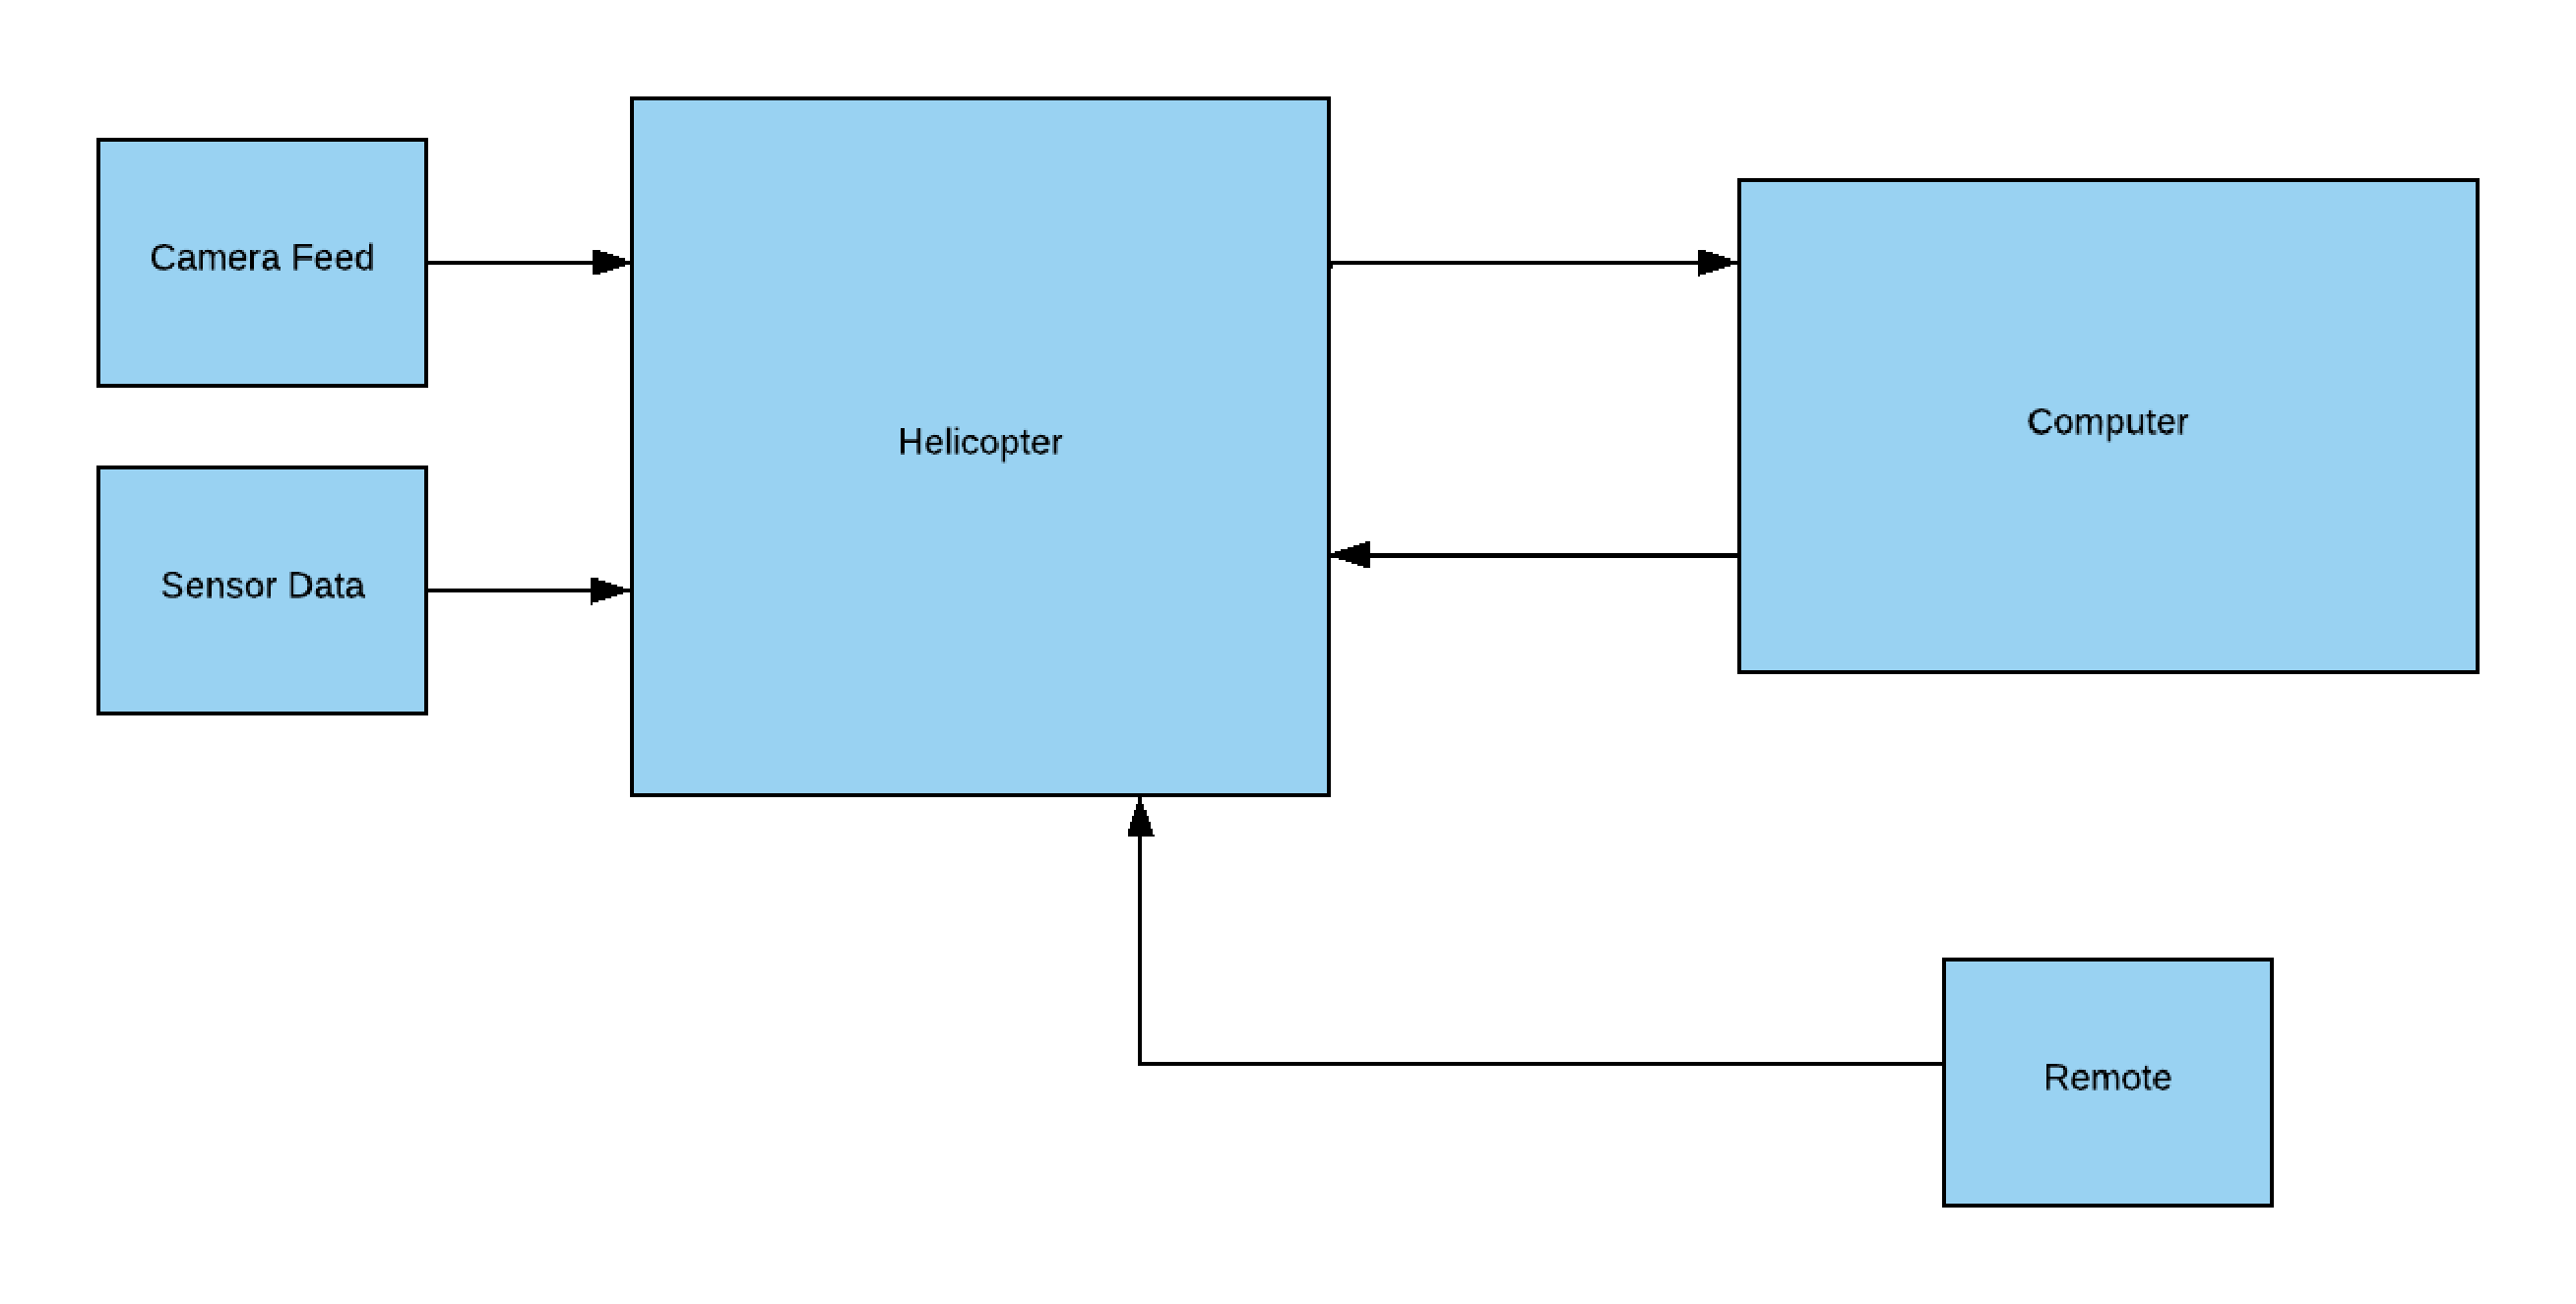
\includegraphics[width=0.7\textwidth]{graphics/high_level_overall_arch.eps}
    \caption{Overall System Software Architecture}
    \label{fig:OverallSystemArchitecture}
\end{figure}

% TODO: Where in this document are we going to define collision avoidance]warning? --Nathan
The responsibilities of the helicopter is to fly through the obstacle course and send data back to the computer. As a part of flying through the course, we want to implement basic collision avoidance on-board the RPi. The RMC will be responsible for a more advanced, more process heavy collision avoidance in the server. \\

The only data that the computer will send to the helicopter is information for collision avoidance, a signal to toggle the collision avoidance being on or off, and a signal to initial the sound system for a victory them. \\

The pilot will operate the movement of a helicopter with a remote but all other externally initiated helicopter signals will be sent from the computer. These external signals will alter the helicopter\textquotesingle s internal state. \\

The cameras, sensors, and computer are the only external systems that will send information to our helicopter module in the Raspberry Pi. The remote will send signals to the helicopter, but those signals will not be feed into the Raspberry Pi to be used by any modules belonging to our subsection of the team.

\subsection{Helicopter}
Our helicopter, operated by a Raspberry Pi Zero and will contain software made in part by us, the Computer Science subsection of the team, and the Electrical Engineer subsection of the team. \\

The diagram below, figure \ref{fig:HelicopterSoftwareArchitecture}, outlines the intended structure of the helicopter\textquotesingle s software. The Raspberry Pi only receives inputs from various sensors, and computer signals from a Wifi transmitter. Outputs are limited to the control of LED lights on the helicopter, operations of the helicopter\textquotesingle s speaker, sending signals to handler motor control, and sending sensor and camera data back to the computer.
% TODO: how should WiFi be capitalized in a formal document? --Nathan

\begin{figure}[h]
    \centering
    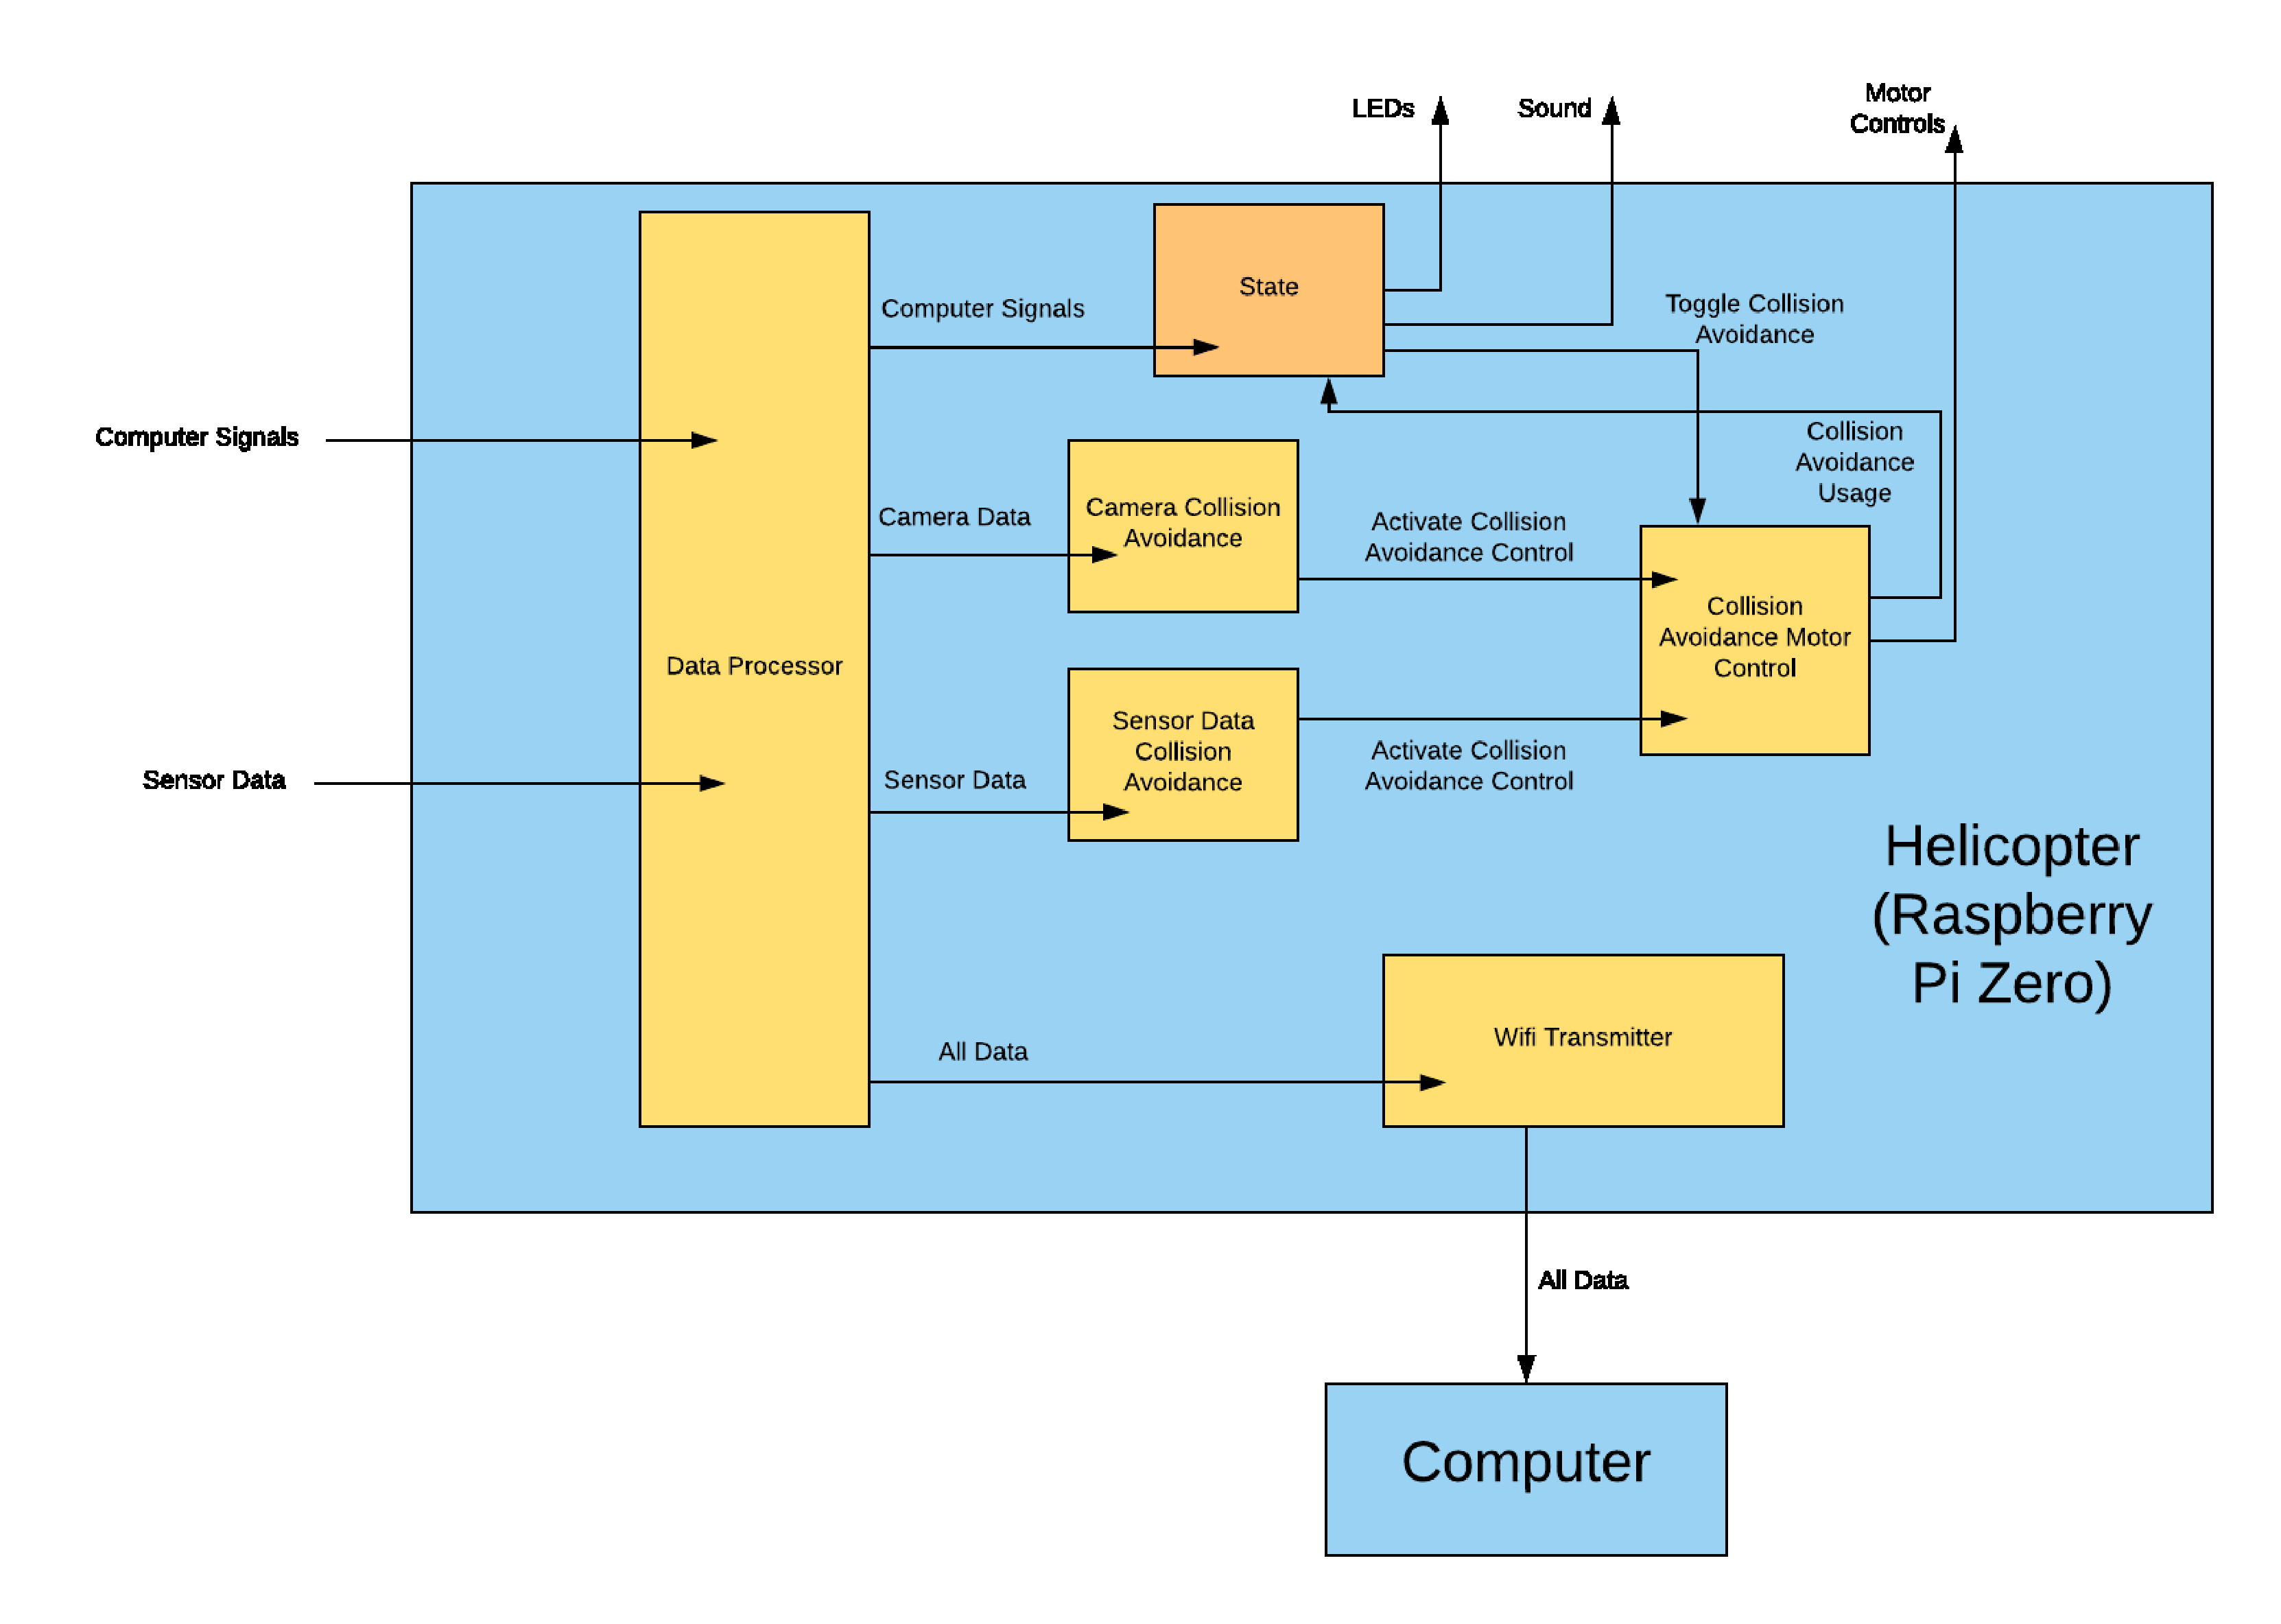
\includegraphics[width=0.9\textwidth]{graphics/helicopter_diagram.eps}
    \caption{Helicopter Software Architecture}
    \label{fig:HelicopterSoftwareArchitecture}
\end{figure}

On-board the helicopter, all incoming signals start by entering into a data processing module which ensures that all incoming data is encapsulated in a format the rest of the system can interpret as opposed to possibly a stream of bytes. The data processor is also responsible for keeping the data sorted and outputting the data in an appropriate, timely fashion. The outgoing data will be sent to four different locations, a state module, a collision avoidance module, based on camera data, a collision avoidance module, based on sensor data, and a transmission module which will be responsible of forwarding data on the helicopter to a computer. \\

The state modules will retain three different types of information, the state of the LEDs, the state of the sound, and a toggle for collision avoidance. The LEDs will have a couple different colors associated with different meanings. The LEDs will initialize to blue, indicating that collision avoidance is on, red will signal the action of collision avoidance, yellow will indicate a collision warning, and green will indicate that collision avoidance is off. Once the course is successful completed, the lights will display a rainbow, initiated by a user activated victory signal from the computer. The same victory signal will update the state to turn the speakers on to play our victory theme. Last, the state module will contain a boolean indicating if collision avoidance is on. This value will be initialized to be on, but upon turning off will signal to the collision avoidance motor control module to not operate on the motors. If this toggle is on, then the collision avoidance motor control will send signals to a motor control unit, implemented by the Electrical Engineer subsection of the team, to impede the pilot from flying the helicopter into an obstacle and a signal will be sent to the state module to indicate that the system is actively using collision avoidance. If the toggle is set to off, the collision avoidance usage signal will be sent as if the toggle was on, but no motor control will take place. Instead, the LEDs will turn yellow to indicate a collision warning instead of the red collision avoidance. \\
% I'm not set on LED color meanings but I just wanted to put something down. --Nathan

There will be two modules that will attempt to calculate collision avoidance separately, one based off a camera depth map, and another based on sensor data. While the internal processing of these modules will occur through different means, both modules will produce the same type of output, a boolean to signal to the collision avoidance motor control module to indicate if collision avoidance should be activated. The collision avoidance motor control module will compare these two incoming values with a logical inclusive or and use that value to attempt collision avoidance or collision warning. \\

To send the camera feeds and various sensor data to the computer the data processor will send the data for a transmitter module. There the data will be sent to a transmitter through an API provided by the Electrical Engineer subsection of our team.

\subsection{Computer}
Our computer view\textquotesingle s main responsibility is to presenting the camera feeds and flight sensor data to the user. The data coming off the helicopter will be sent to a server running locally on the computer. This server, in addition to serving the viewing page, will compute collision avoidance and collision warning for displaying to the user. The view will also capture various keyboard inputs to signal to the server to signal to the helicopter to toggle collision avoidance, and signal victory lights and sounds.

\begin{figure}[h]
    \centering
    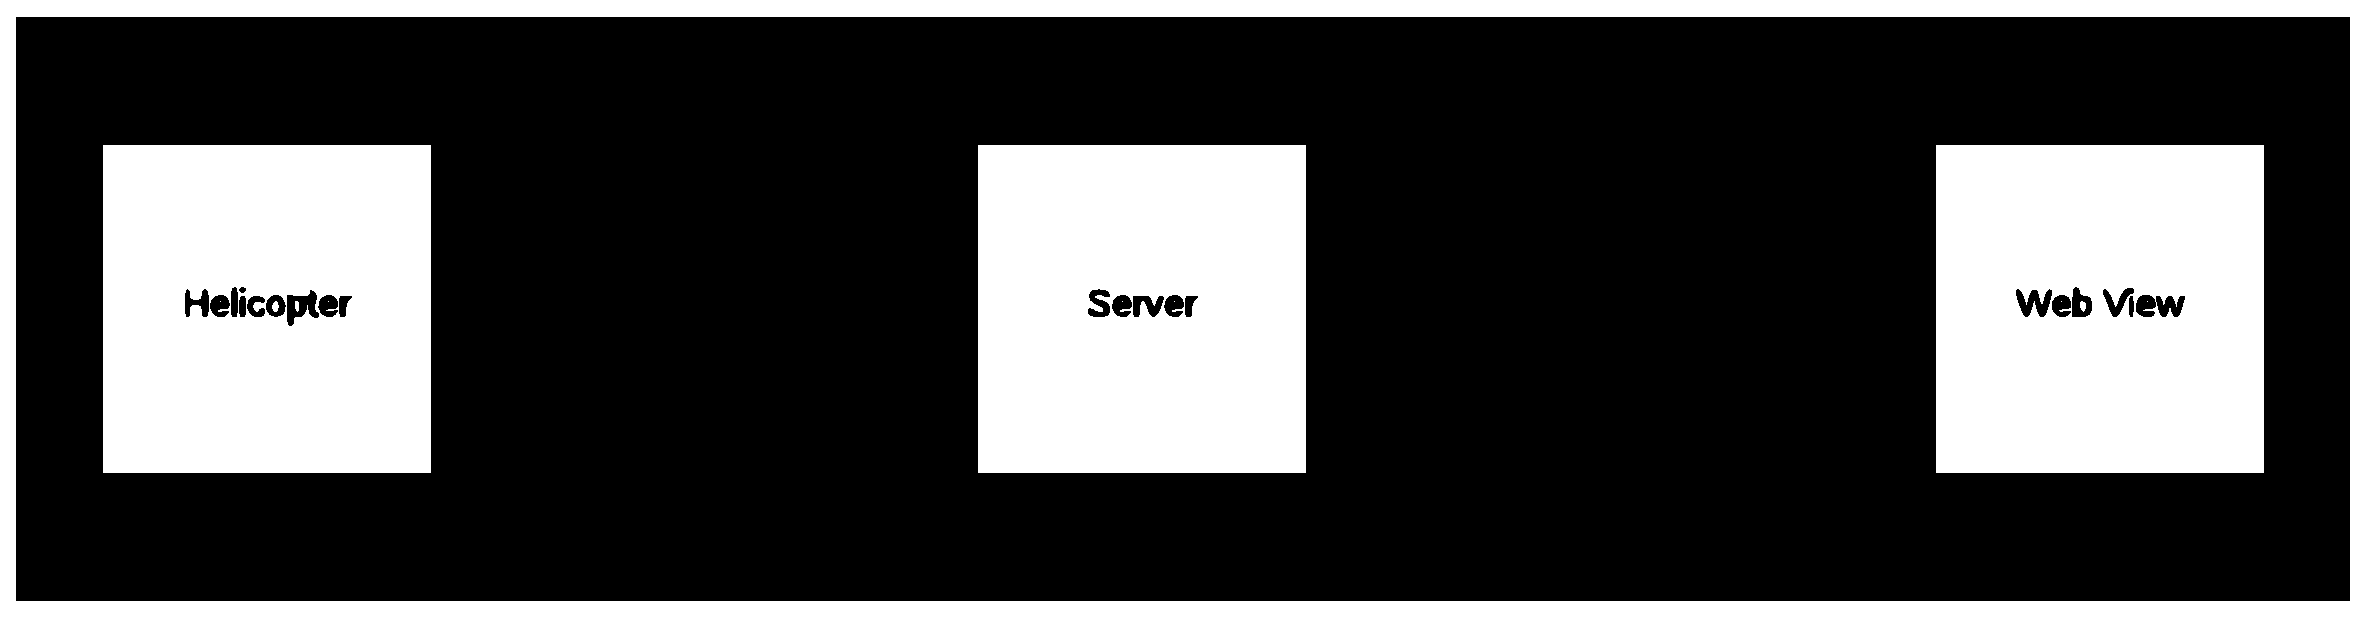
\includegraphics[width=0.8\textwidth]{graphics/computer_diagram.eps}
    \caption{Computer View Software Architecture}
    \label{fig:ComputerViewSoftwareArchitecture}
\end{figure}

\section{Component Design}
The following section describes software and their required components for the Raspberry Pi on-board the MAV and for a separate computer.

\subsection{Image Recognition}
\subsubsection{Introduction}
Computer Vision is an essential portion of the remote-controlled helicopter that enables the pilot to view and detect obstacles that may appear in its path. The American Helicopter Society competition contains a course with obstacles such as walls, trees, and bridges. Additionally, a part of the course cannot be seen through human eyes, so the helicopter must solely rely on a camera. Computer Vision will allow the pilot to have other intelligence data that can assist in avoiding obstacles. After exploring several image recognition APIs such as OpenCV, Amazon Recognition, and Google Cloud Vision, our team has chosen OpenCV because of the real-time image recognition benefits and it is a low-cost option.

\subsubsection{OpenCV}
OpenCV, which stands for Open Computer Vision, is an open source library that gives access to numerous capabilities to efficiently detect objects. OpenCV has various inbuilt functions that allow a user to inference objects and perform actions quickly. Since OpenCV is a software development kit, the inferencing and machine learning must be performed on the local machine as there is no cloud option available. Additionally, OpenCV allows us to detect and recognize objects in real-time, so it is the chose API for our product. Specifically, we will be using OpenCV on the bottom-facing camera to find an optimal pickup point for the payload. Figure \ref{fig:ObjectRecognitionWorkflow} explains the general workflow we will be using to leverage machine learning methods to navigate the pilot of the optimal pickup point. \\

\begin{figure}[h!]
    \centering
    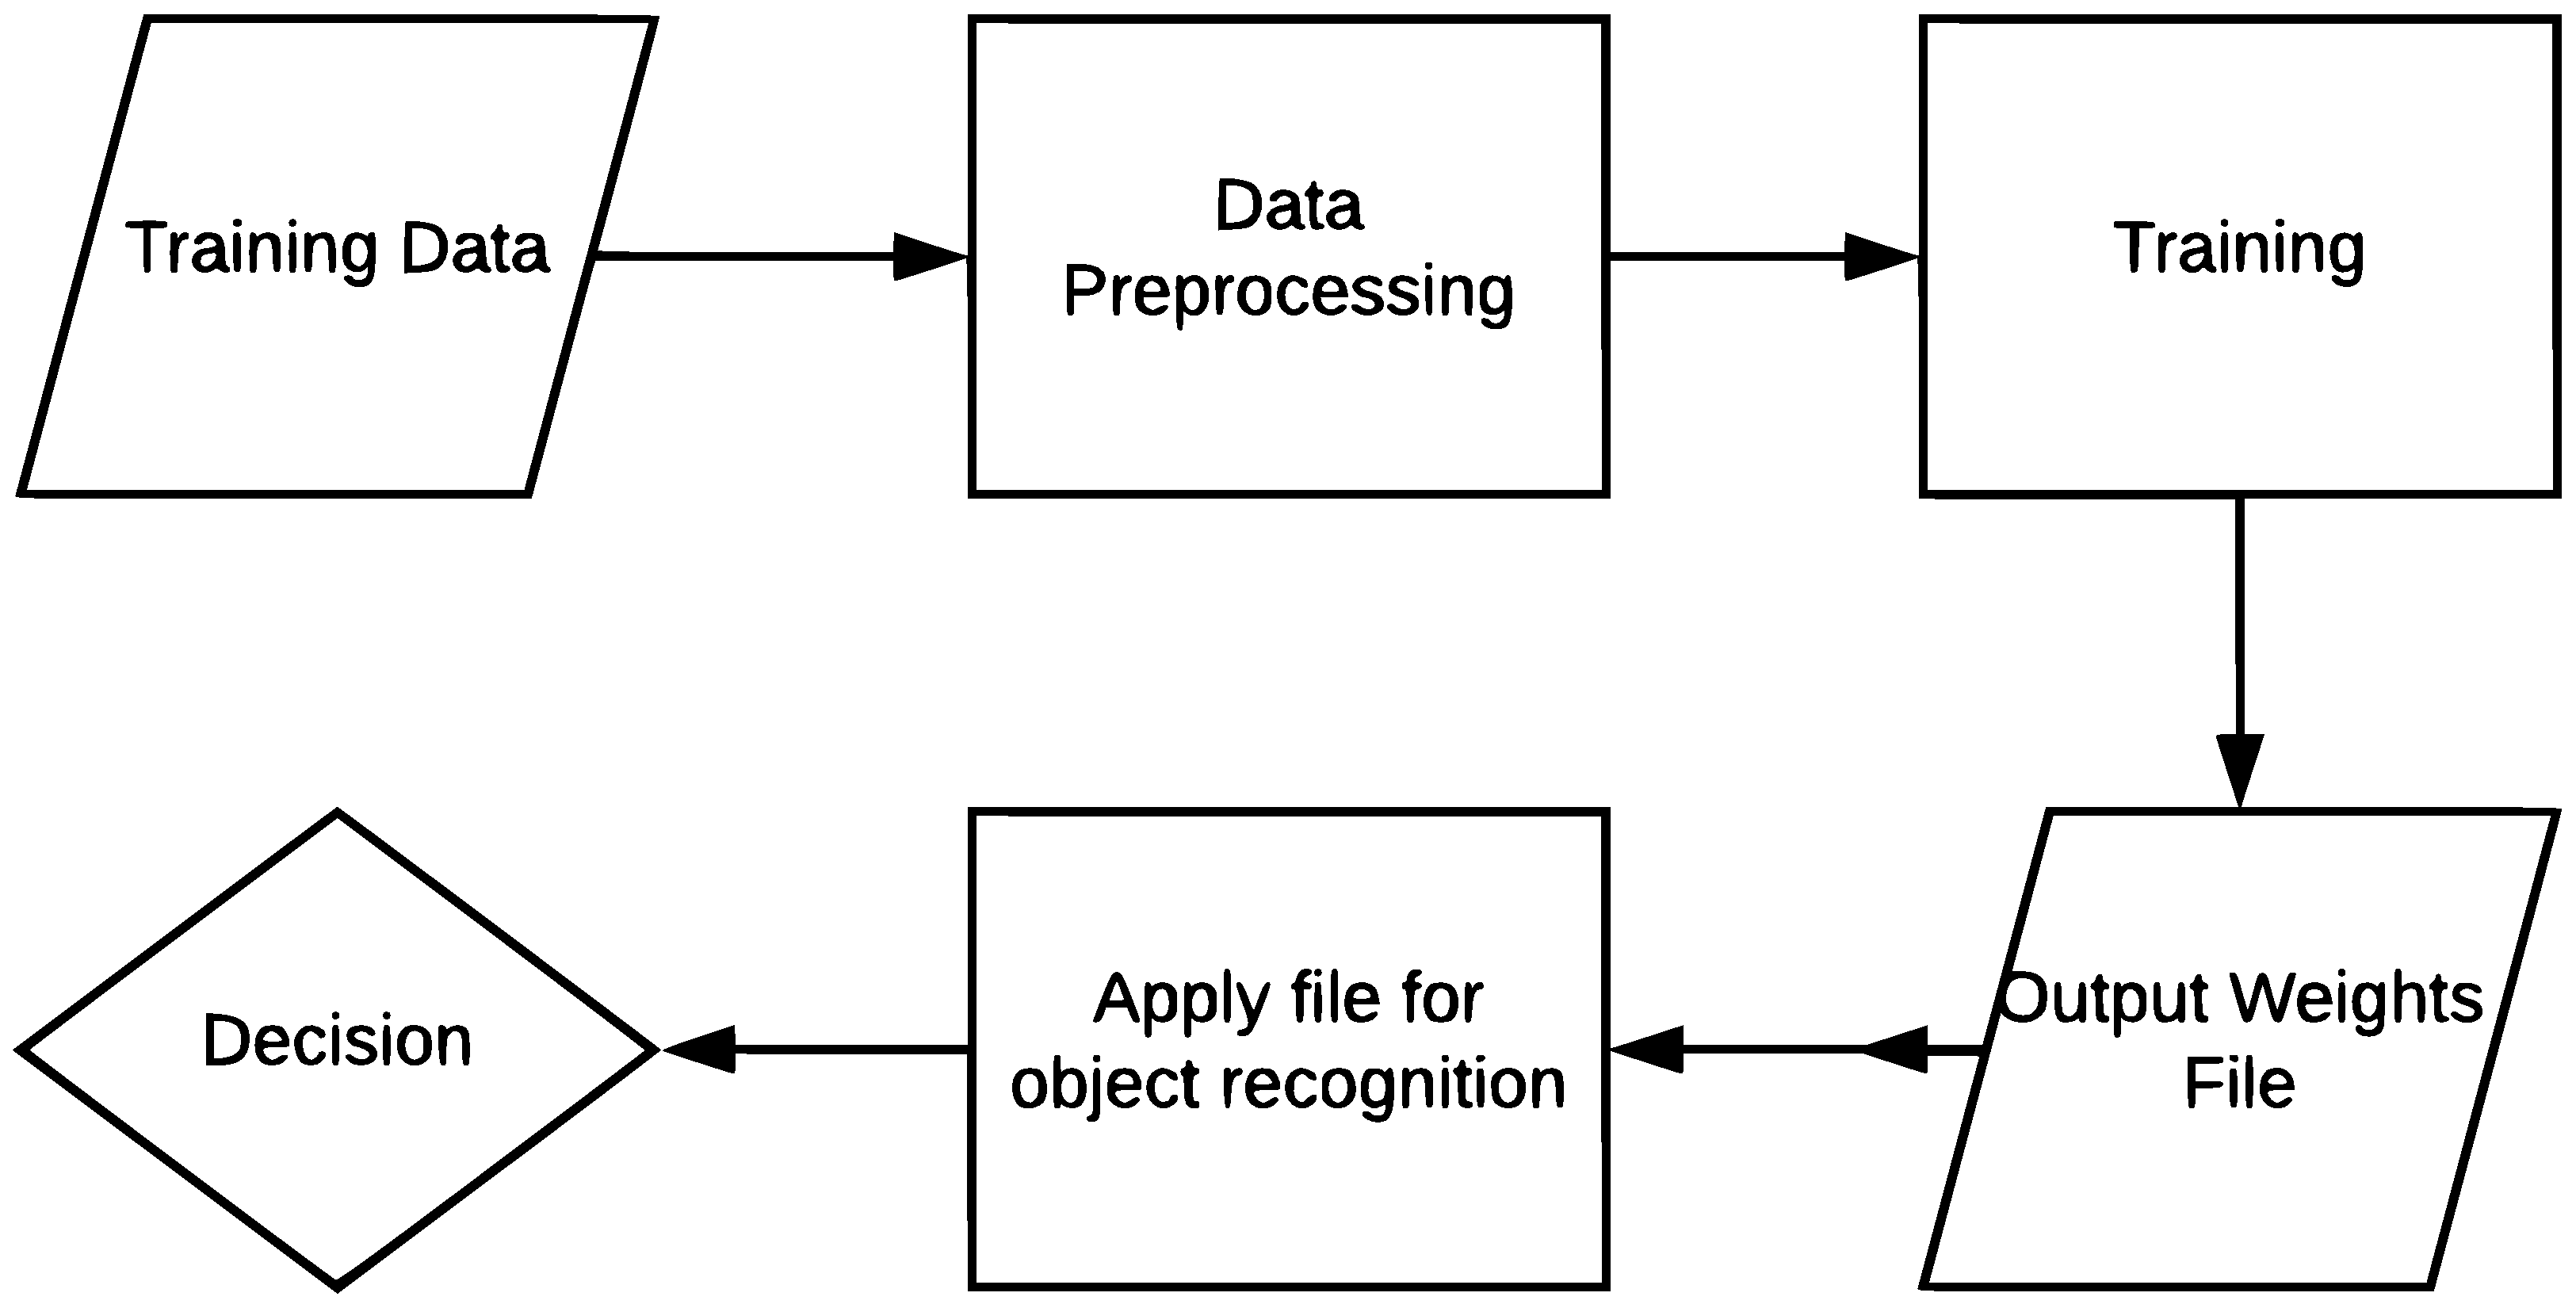
\includegraphics[width=0.5\textwidth]{graphics/object_recognition_workflow.eps}
    \caption{Object Recognition Workflow}
    \label{fig:ObjectRecognitionWorkflow}
\end{figure}

Each of the components performs a significant task in developing an intelligent platform to detect the pickup points.
\begin{itemize}
    \item Training Data: Gather image data of the payload pickup and drop-off point based on the competition information.
    \item Data Preprocessing: Before data, the data needed to be cleaned to a unified structure that allows for equal learning opportunities to learn.
    \item Training: Training the image data is a critical portion of image recognition. The training segment is where the machine learns to distinguish between different objects.
    \item Neural Network: The current design choice is to build a neural network, which is a deep learning mechanism to train our model. While computationally expensive, a neural network generally yields accurate results when inferencing an object.
    \item Output Weights File: The weights file is the multidimensional output from the training. It is the neural network connections that were generated in order to achieve accurate inferencing.
    \item Using Weight file for object recognition: Once the weight file is ready from the training, we load the file into the computer vision application which enables the inferencing.
    \item Decision: Finally, the local machine has the ability to detect objects in real-time (in this scenario, we now have the ability to find an optimal payload pickup point).
\end{itemize}

After the above components are implemented, a computer can begin to inference objects and provide extra intelligence, such as the distance to the optimal pickup point as well as the target location. The video feed of the computer vision application will be displayed on the Graphical User Interface (GUI) will be discussed later.

\subsubsection{Design Rationale}
After high consideration, our team chose to implement computer vision technology for the bottom-facing camera to assist the pilot while picking up the package. In the previous years, payload pickup was a challenging component of the competition. Teams often lose the most time when picking up and dropping off a package because they are unable to find an efficient point to disembark and load the package. The machine learning technology onboard to intended to help the pilot navigate to a position which is easiest for pickup. \\

While computationally expensive, the Electrical Engineering and the Computer Science teams met to discuss methods to prevent excessively draining the battery due to the real-time inferencing. Our conclusion was to pipe off the data from the transmitter into a local machine and have the image recognition component be done on a computer.


\subsection{Collision Warning}
\subsubsection{Introduction}
Collision warning enhances pilot\textquotesingle s awareness of the surroundings, including outside the field of view provided by the camera. To inform the pilot of obstacles surrounding the perimeter of the MAV, we implement a collision warning system.

\subsubsection{Structure}
The system involves three \textit{LV-MaxSonar-EZ0} ultrasonic range sensors, with one at the front and two at the sides of the MAV. Due to the scarcity of available power and an imposed mass limit requirement, a range sensor at the rear of the MAV is not included. The range sensors detect obstacles within a conical-like field of view. Whenever the MAV is close to the ground, there is a chance for the ground itself to be treated as an obstacle. Utilizing a bottom facing range sensor will allow for temporarily turning off collision warning system whenever the MAV is near the surface of the terrain. \\

Collision warning system is established at the server side. Range sensor data received from the MAV is processed at the server side and reflected in the web page, as noted in figure \ref{fig:ColWar}.
\begin{figure}[h]
    \centering
    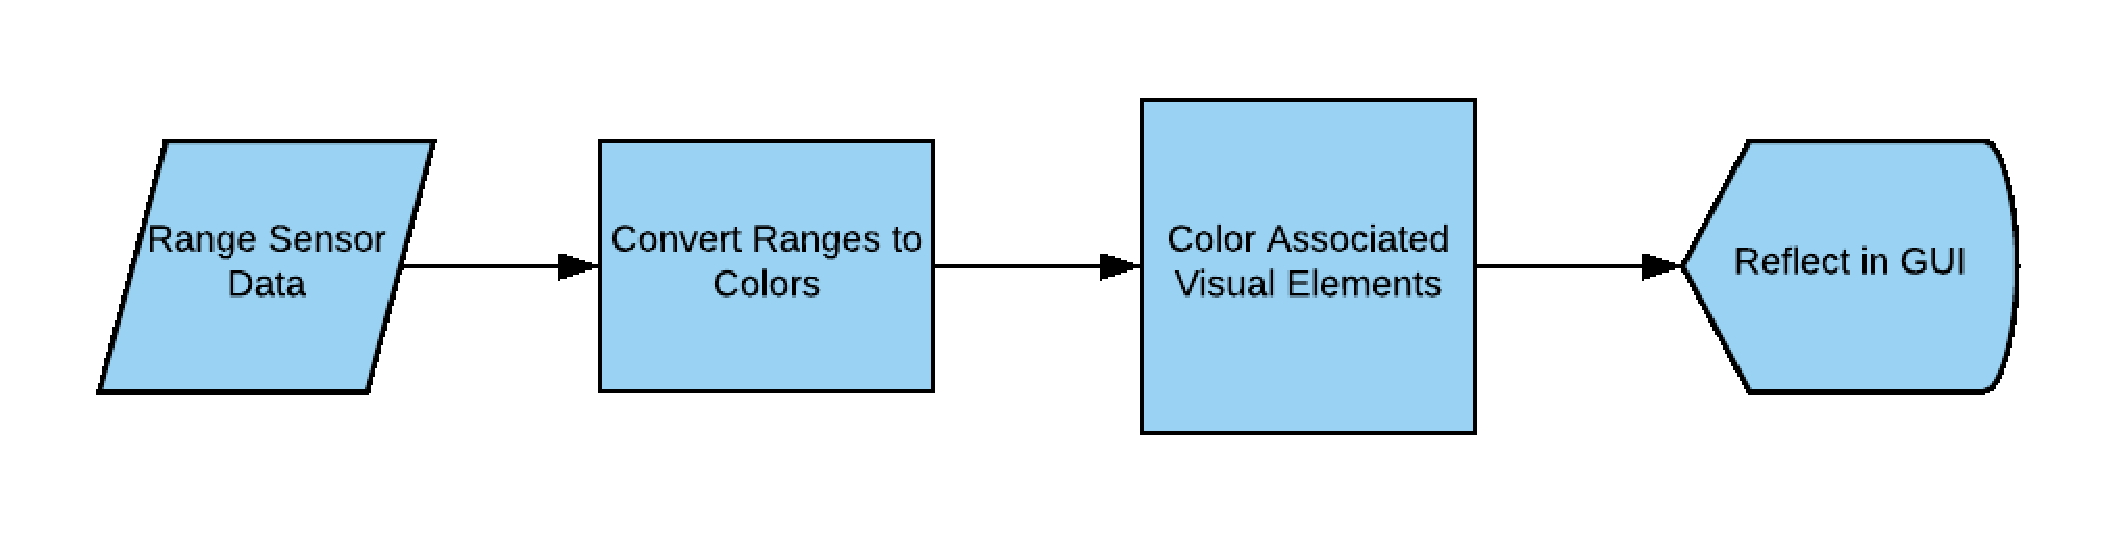
\includegraphics[height=3.5cm]{graphics/collision_warning.eps}
    \caption{Collision Warning Flow}
    \label{fig:ColWar}
\end{figure}

\subsubsection{GUI Element}
The GUI consists of a top view of the MAV, surrounded by colored semi-pie sections, shown in figure \ref{fig:ColWarGUI}. Each pie section is dedicated to its associated range sensor and is colored in green, yellow, orange, or red, depending on how far an obstacle is. Red indicates obstacle is too close and green indicates no obstacles within a safe radius.
\begin{figure}[h]
    \centering
    
\includegraphics[height=3.5cm]{graphics/collision_warning_gui.eps}
    \caption{Collision Warning GUI}
    \label{fig:ColWarGUI}
\end{figure}

\subsubsection{Design Rationale}
The design concept was acquired from the visual display of the road vehicle parking assist software. This allows for the pilot to see where the helicopter is located with respect to obstacles.

\subsection{Collision Avoidance}
\subsubsection{Introduction}
Collision avoidance is collision warning at the next level. Whenever the MAV is too close to an obstacle, the collision avoidance system overrides controls to prevent the MAV from moving further toward the obstacle. Additionally, the collision avoidance computes proper rejection pitch and roll components to ensure that the MAV does not keep moving in the direction of an obstacle.

\subsubsection{Structure}
Collision avoidance involves all the range sensors, accelerometer, and potentially the depth map from the front facing camera. For rapid response, collision avoidance is processed onboard the MAV. Figure \ref{fig:ColAvo} shows the onbaord collision system implementation.
\begin{figure}[h]
    \centering
    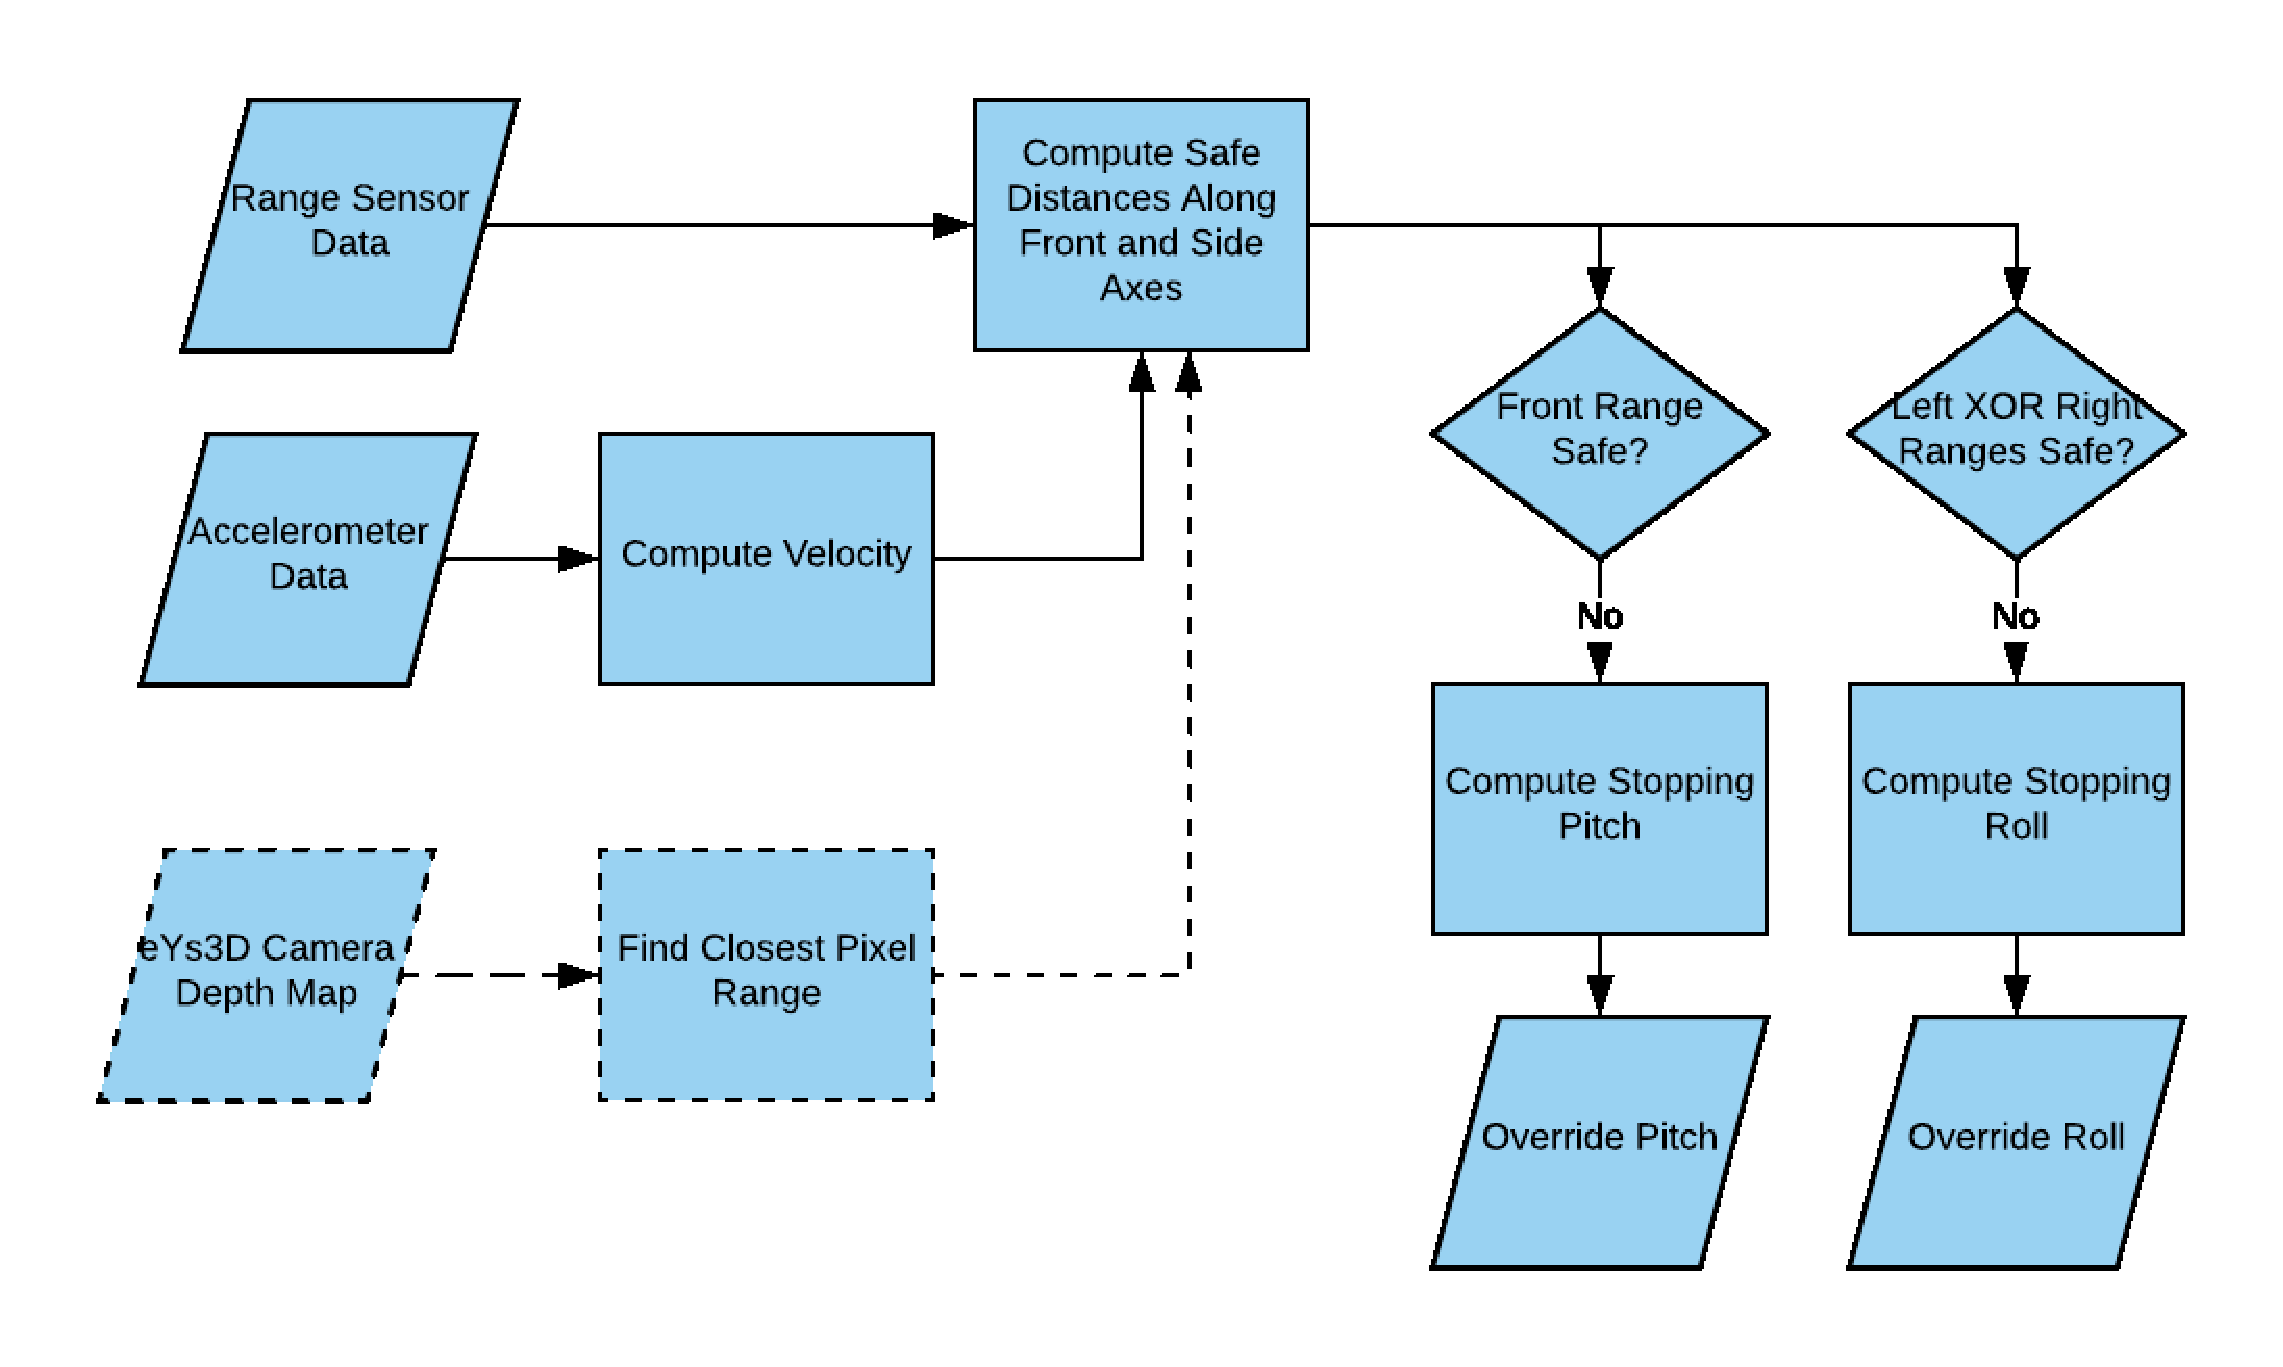
\includegraphics[width=0.8\textwidth]{graphics/collision_avoidance.eps}
    \caption{Collision Avoidance}
    \label{fig:ColAvo}
\end{figure}

Depth map from camera data can also assist in collision avoidance; however, due to processing requirement the entire depth map may have to be shipped off to the sever, processed at the sever, and if collision override is required, new pitch and roll controls are transmitted to the MAV.

\subsubsection{Remote Switch}
As part of the VFS requirements, the remote must have a kill switch to disable autonomous operations. A switch on the remote and a dedicated channel will allow for the pilot to toggle collision avoidance.

\subsubsection{GUI Element}
For reference, the GUI will have a text box or a light, indicating whether collision avoidance is turned on or turned off.

\subsubsection{Design Rationale}
In order for the pilot to be certain that collision avoidance is turned off, it must be clearly indicated in the GUI. A bold text or a labeled circle element colored in black or green would be a viable solution.

\subsection{Height Detection}
\subsubsection{Introduction}
Height detection allows for utilizing features, including package pickup assist, collision avoidance, and GUI feedback for the pilot regarding how high the MAV is from the surface of the terrain.

\subsubsection{Structure}
To inform the pilot of the height, bottom range sensor data acquired from the MAV is transmitted to the server, where it is rounded up and written to a text input element within the GUI.

\subsubsection{GUI Element}
For the pilot to be aware of the height, a label element, \textit{Height}, along with a height value next to the label is included. Potential positions for the label, within the GUI, include upper left or lower right corners.

\subsubsection{Design Rationale}
Because height is only important during package pickup, the height text box should not stand out on the screen during normal flight operations. It can, however, stand out, or even be displayed in an alternative fashion, when pickup assist mode is turned on.

\subsection{Pickup Guidance}
\subsubsection{Introduction}
Alignment over the package is crucial and is the primary step required to be achived for package pickup. A package guidanance visual indicator is therefore included.

\subsubsection{Structure}
Bottom facing camera feed, gyroscope data, and height sensor data acquired from the MAV is processed at the server side and converted to a visual display.

\subsubsection{GUI Element}
Two components with top view and side view are necessary for package pickup. The top view provides planar alignment of the MAV over the package. The side view provides vertical alignment, vertical tilt, and height over the package.

\subsubsection{Design Rationale}
Whenever the pilot is to pickup a package, the best way for them to align over the package is have a top view, from above the MAV, and a side view, from the side of the MAV. Because camera view over the MAV is not possible, the bottom-facing camera below the MAV, along with graphics reference of the MAV over the video stream, will allow for the pilot to align properly over the package. For the side view, a simple graphic is be made to represent the MAV alignment over the package.

\subsection{Attitude Indicator}
\subsubsection{Introduction}
Vertical alignment awareness allows for the pilot to know how the MAV is aligned with respect to horizontal.

\subsubsection{Structure}
Data provided from the gyroscope is processed and converted to a horizon alignment visual.

\subsubsection{GUI Element}
An attitude indicator appearing at the bottom-left corner of the GUI.

\subsubsection{Design Rationale}
All manual controlled aviation vehicles have attitude instrument. It is beneficial for the MAV pilot to have access to this data as well.

\subsection{Speed Indicator}
\subsubsection{Introduction}
Although speed indicator is not a crucial component, presenting the flight variable to the pilot allows for the pilot to keep track of the velocity.

\subsubsection{Structure}
Accelerometer data acquired from the MAV is processed at the server and converted to velocity along all axes. Front, side, and vertical speed are then fed to the GUI.

\subsubsection{GUI Element}
Three speed labels and their values are displayed at the bottom-center view of the GUI. Speeds along the three axes are displayed in a text form.

\subsubsection{Design Rationale}
Presenting speed in text form is enough for the pilot to be aware of how fast the MAV is moving. Additionally, velocity is not an important indicator and therefore must take minimal space on the main screen.

\subsection{Front Video Feed}
\subsubsection{Introduction}
Front camera video feed is the most essential and a required component of the design.

\subsubsection{GUI Element}
A background window element with video feed overlaying the entire element area.

\subsubsection{Design Rationale}
Because video feed is a required component and allows for the pilot to see what the MAV is doing whenever the MAV is not visible to the pilot, the entire video feed should stand out. Overlaying the entire monitor provides a clear visual to the pilot.

\subsection{Bottom Video Feed}
\subsubsection{Introduction}
Bottom facing video feed provides additional visual information to the pilot, including is used to assist the pilot in package pickup. The video feed may be overlayed with image recognition and package assist components.

\subsubsection{GUI Element}
A smaller rectangular area at the right side of the screen, displaying the bottom camera video feed. Whenever the pickup mode is entered, the rectangular area is enlarged and additional pickup assist elements are displayed in the rectangular area.

\subsubsection{Design Rational}
Because bottom video feed is not as important as the  front video feed, the rectangular area for the bottom video feed must not stand out.

\subsection{LED Control}
\subsubsection{Introduction}
The MAV is equipped with LEDs and their flashing and color is controlled by script.

\subsubsection{Structure}
The server processes flight variables and transmits color and brightness of LEDs to the MAV.

\subsection{Speaker Control}
\subsubsection{Introduction}
The speaker at the MAV is to provide auditory feedback to the pilot and the entire group at the competition, including the victory song, and collision avoidance mode switch.

\subsubsection{Structure}
The server processes acquired information from the MAV and determines when to play sounds and which sounds to play, which is then transmitted to the MAV to trigger the on-board speaker. The sounds and music themselves may very likely be stored on-board the MAV. The server transmits the identifier of the sound to trigger.

\section{User Interface}
The graphical user interface consists of a web-page, with the entire background covered with a front view video feed. Flight instrument component elements and bottom facing camera feed element overlay the sides of the main video feed and may be semi-transparent. When package pickup mode is entered, the bottom facing camera feed window is enlarge sightly and pickup guidance elements are presented. Shown in figure \ref{fig:UI} is a mock-up of the GUI. All GUI elements, except for the flight variables, are explanatory. The flight variables section provides the pilot with height, velocity, forward tilt, and a any other non-essential variables.

\begin{figure}[h]
    \centering
    
\includegraphics[width=0.9\textwidth]{graphics/ui.eps}
    \caption{Graphical User Interface}
    \label{fig:UI}
\end{figure}

\clearpage
\medskip
\bibliographystyle{IEEEtran}
\bibliography{ref}
\end{document}
